% GNUPLOT: LaTeX picture with Postscript
\begingroup
  \makeatletter
  \providecommand\color[2][]{%
    \GenericError{(gnuplot) \space\space\space\@spaces}{%
      Package color not loaded in conjunction with
      terminal option `colourtext'%
    }{See the gnuplot documentation for explanation.%
    }{Either use 'blacktext' in gnuplot or load the package
      color.sty in LaTeX.}%
    \renewcommand\color[2][]{}%
  }%
  \providecommand\includegraphics[2][]{%
    \GenericError{(gnuplot) \space\space\space\@spaces}{%
      Package graphicx or graphics not loaded%
    }{See the gnuplot documentation for explanation.%
    }{The gnuplot epslatex terminal needs graphicx.sty or graphics.sty.}%
    \renewcommand\includegraphics[2][]{}%
  }%
  \providecommand\rotatebox[2]{#2}%
  \@ifundefined{ifGPcolor}{%
    \newif\ifGPcolor
    \GPcolortrue
  }{}%
  \@ifundefined{ifGPblacktext}{%
    \newif\ifGPblacktext
    \GPblacktexttrue
  }{}%
  % define a \g@addto@macro without @ in the name:
  \let\gplgaddtomacro\g@addto@macro
  % define empty templates for all commands taking text:
  \gdef\gplbacktext{}%
  \gdef\gplfronttext{}%
  \makeatother
  \ifGPblacktext
    % no textcolor at all
    \def\colorrgb#1{}%
    \def\colorgray#1{}%
  \else
    % gray or color?
    \ifGPcolor
      \def\colorrgb#1{\color[rgb]{#1}}%
      \def\colorgray#1{\color[gray]{#1}}%
      \expandafter\def\csname LTw\endcsname{\color{white}}%
      \expandafter\def\csname LTb\endcsname{\color{black}}%
      \expandafter\def\csname LTa\endcsname{\color{black}}%
      \expandafter\def\csname LT0\endcsname{\color[rgb]{1,0,0}}%
      \expandafter\def\csname LT1\endcsname{\color[rgb]{0,1,0}}%
      \expandafter\def\csname LT2\endcsname{\color[rgb]{0,0,1}}%
      \expandafter\def\csname LT3\endcsname{\color[rgb]{1,0,1}}%
      \expandafter\def\csname LT4\endcsname{\color[rgb]{0,1,1}}%
      \expandafter\def\csname LT5\endcsname{\color[rgb]{1,1,0}}%
      \expandafter\def\csname LT6\endcsname{\color[rgb]{0,0,0}}%
      \expandafter\def\csname LT7\endcsname{\color[rgb]{1,0.3,0}}%
      \expandafter\def\csname LT8\endcsname{\color[rgb]{0.5,0.5,0.5}}%
    \else
      % gray
      \def\colorrgb#1{\color{black}}%
      \def\colorgray#1{\color[gray]{#1}}%
      \expandafter\def\csname LTw\endcsname{\color{white}}%
      \expandafter\def\csname LTb\endcsname{\color{black}}%
      \expandafter\def\csname LTa\endcsname{\color{black}}%
      \expandafter\def\csname LT0\endcsname{\color{black}}%
      \expandafter\def\csname LT1\endcsname{\color{black}}%
      \expandafter\def\csname LT2\endcsname{\color{black}}%
      \expandafter\def\csname LT3\endcsname{\color{black}}%
      \expandafter\def\csname LT4\endcsname{\color{black}}%
      \expandafter\def\csname LT5\endcsname{\color{black}}%
      \expandafter\def\csname LT6\endcsname{\color{black}}%
      \expandafter\def\csname LT7\endcsname{\color{black}}%
      \expandafter\def\csname LT8\endcsname{\color{black}}%
    \fi
  \fi
    \setlength{\unitlength}{0.0500bp}%
    \ifx\gptboxheight\undefined%
      \newlength{\gptboxheight}%
      \newlength{\gptboxwidth}%
      \newsavebox{\gptboxtext}%
    \fi%
    \setlength{\fboxrule}{0.5pt}%
    \setlength{\fboxsep}{1pt}%
    \definecolor{tbcol}{rgb}{1,1,1}%
\begin{picture}(9060.00,7360.00)%
    \gplgaddtomacro\gplbacktext{%
      \csname LTb\endcsname%%
      \put(598,4176){\makebox(0,0)[r]{\strut{}$15$}}%
      \csname LTb\endcsname%%
      \put(598,4624){\makebox(0,0)[r]{\strut{}$15.5$}}%
      \csname LTb\endcsname%%
      \put(598,5072){\makebox(0,0)[r]{\strut{}$16$}}%
      \csname LTb\endcsname%%
      \put(598,5520){\makebox(0,0)[r]{\strut{}$16.5$}}%
      \csname LTb\endcsname%%
      \put(598,5968){\makebox(0,0)[r]{\strut{}$17$}}%
      \csname LTb\endcsname%%
      \put(598,6416){\makebox(0,0)[r]{\strut{}$17.5$}}%
      \csname LTb\endcsname%%
      \put(598,6864){\makebox(0,0)[r]{\strut{}$18$}}%
      \csname LTb\endcsname%%
      \put(679,4018){\makebox(0,0){\strut{}0.0$\times10^{0}$}}%
      \csname LTb\endcsname%%
      \put(1129,4018){\makebox(0,0){\strut{}2.0$\times10^{5}$}}%
      \csname LTb\endcsname%%
      \put(1579,4018){\makebox(0,0){\strut{}4.0$\times10^{5}$}}%
      \csname LTb\endcsname%%
      \put(2029,4018){\makebox(0,0){\strut{}6.0$\times10^{5}$}}%
      \csname LTb\endcsname%%
      \put(2479,4018){\makebox(0,0){\strut{}8.0$\times10^{5}$}}%
      \csname LTb\endcsname%%
      \put(2929,4018){\makebox(0,0){\strut{}1.0$\times10^{6}$}}%
      \csname LTb\endcsname%%
      \put(3379,4018){\makebox(0,0){\strut{}1.2$\times10^{6}$}}%
      \csname LTb\endcsname%%
      \put(3829,4018){\makebox(0,0){\strut{}1.4$\times10^{6}$}}%
      \csname LTb\endcsname%%
      \put(4279,4018){\makebox(0,0){\strut{}1.6$\times10^{6}$}}%
    }%
    \gplgaddtomacro\gplfronttext{%
      \csname LTb\endcsname%%
      \put(139,5520){\rotatebox{-270.00}{\makebox(0,0){\strut{}Resistance (Pa/(L/min))}}}%
      \csname LTb\endcsname%%
      \put(2479,3780){\makebox(0,0){\strut{}Number of volume cells}}%
      \csname LTb\endcsname%%
      \put(2479,7102){\makebox(0,0){\strut{}Resistance (Pa/(L/min))}}%
    }%
    \gplgaddtomacro\gplbacktext{%
      \csname LTb\endcsname%%
      \put(5199,4176){\makebox(0,0)[r]{\strut{}$73.35$}}%
      \csname LTb\endcsname%%
      \put(5199,4560){\makebox(0,0)[r]{\strut{}$73.4$}}%
      \csname LTb\endcsname%%
      \put(5199,4944){\makebox(0,0)[r]{\strut{}$73.45$}}%
      \csname LTb\endcsname%%
      \put(5199,5328){\makebox(0,0)[r]{\strut{}$73.5$}}%
      \csname LTb\endcsname%%
      \put(5199,5712){\makebox(0,0)[r]{\strut{}$73.55$}}%
      \csname LTb\endcsname%%
      \put(5199,6096){\makebox(0,0)[r]{\strut{}$73.6$}}%
      \csname LTb\endcsname%%
      \put(5199,6480){\makebox(0,0)[r]{\strut{}$73.65$}}%
      \csname LTb\endcsname%%
      \put(5199,6864){\makebox(0,0)[r]{\strut{}$73.7$}}%
      \csname LTb\endcsname%%
      \put(5279,4018){\makebox(0,0){\strut{}0.0$\times10^{0}$}}%
      \csname LTb\endcsname%%
      \put(5719,4018){\makebox(0,0){\strut{}2.0$\times10^{5}$}}%
      \csname LTb\endcsname%%
      \put(6159,4018){\makebox(0,0){\strut{}4.0$\times10^{5}$}}%
      \csname LTb\endcsname%%
      \put(6599,4018){\makebox(0,0){\strut{}6.0$\times10^{5}$}}%
      \csname LTb\endcsname%%
      \put(7039,4018){\makebox(0,0){\strut{}8.0$\times10^{5}$}}%
      \csname LTb\endcsname%%
      \put(7479,4018){\makebox(0,0){\strut{}1.0$\times10^{6}$}}%
      \csname LTb\endcsname%%
      \put(7919,4018){\makebox(0,0){\strut{}1.2$\times10^{6}$}}%
      \csname LTb\endcsname%%
      \put(8359,4018){\makebox(0,0){\strut{}1.4$\times10^{6}$}}%
      \csname LTb\endcsname%%
      \put(8799,4018){\makebox(0,0){\strut{}1.6$\times10^{6}$}}%
    }%
    \gplgaddtomacro\gplfronttext{%
      \csname LTb\endcsname%%
      \put(4659,5520){\rotatebox{-270.00}{\makebox(0,0){\strut{}Right-lung flow fraction (\%)}}}%
      \csname LTb\endcsname%%
      \put(7039,3780){\makebox(0,0){\strut{}Number of volume cells}}%
      \csname LTb\endcsname%%
      \put(7039,7102){\makebox(0,0){\strut{}Right-lung flow fraction (\%)}}%
    }%
    \gplgaddtomacro\gplbacktext{%
      \csname LTb\endcsname%%
      \put(598,506){\makebox(0,0)[r]{\strut{}$15.2$}}%
      \csname LTb\endcsname%%
      \put(598,954){\makebox(0,0)[r]{\strut{}$15.4$}}%
      \csname LTb\endcsname%%
      \put(598,1402){\makebox(0,0)[r]{\strut{}$15.6$}}%
      \csname LTb\endcsname%%
      \put(598,1850){\makebox(0,0)[r]{\strut{}$15.8$}}%
      \csname LTb\endcsname%%
      \put(598,2298){\makebox(0,0)[r]{\strut{}$16$}}%
      \csname LTb\endcsname%%
      \put(598,2746){\makebox(0,0)[r]{\strut{}$16.2$}}%
      \csname LTb\endcsname%%
      \put(598,3194){\makebox(0,0)[r]{\strut{}$16.4$}}%
      \csname LTb\endcsname%%
      \put(679,348){\makebox(0,0){\strut{}0.0$\times10^{0}$}}%
      \csname LTb\endcsname%%
      \put(1129,348){\makebox(0,0){\strut{}2.0$\times10^{5}$}}%
      \csname LTb\endcsname%%
      \put(1579,348){\makebox(0,0){\strut{}4.0$\times10^{5}$}}%
      \csname LTb\endcsname%%
      \put(2029,348){\makebox(0,0){\strut{}6.0$\times10^{5}$}}%
      \csname LTb\endcsname%%
      \put(2479,348){\makebox(0,0){\strut{}8.0$\times10^{5}$}}%
      \csname LTb\endcsname%%
      \put(2929,348){\makebox(0,0){\strut{}1.0$\times10^{6}$}}%
      \csname LTb\endcsname%%
      \put(3379,348){\makebox(0,0){\strut{}1.2$\times10^{6}$}}%
      \csname LTb\endcsname%%
      \put(3829,348){\makebox(0,0){\strut{}1.4$\times10^{6}$}}%
      \csname LTb\endcsname%%
      \put(4279,348){\makebox(0,0){\strut{}1.6$\times10^{6}$}}%
    }%
    \gplgaddtomacro\gplfronttext{%
      \csname LTb\endcsname%%
      \put(139,1850){\rotatebox{-270.00}{\makebox(0,0){\strut{}Right-superior share of right flow (\%)}}}%
      \csname LTb\endcsname%%
      \put(2479,110){\makebox(0,0){\strut{}Number of volume cells}}%
      \csname LTb\endcsname%%
      \put(2479,3432){\makebox(0,0){\strut{}Right-superior share of right flow (\%)}}%
    }%
    \gplgaddtomacro\gplbacktext{%
      \csname LTb\endcsname%%
      \put(5118,506){\makebox(0,0)[r]{\strut{}$9.4$}}%
      \csname LTb\endcsname%%
      \put(5118,805){\makebox(0,0)[r]{\strut{}$9.45$}}%
      \csname LTb\endcsname%%
      \put(5118,1104){\makebox(0,0)[r]{\strut{}$9.5$}}%
      \csname LTb\endcsname%%
      \put(5118,1402){\makebox(0,0)[r]{\strut{}$9.55$}}%
      \csname LTb\endcsname%%
      \put(5118,1701){\makebox(0,0)[r]{\strut{}$9.6$}}%
      \csname LTb\endcsname%%
      \put(5118,2000){\makebox(0,0)[r]{\strut{}$9.65$}}%
      \csname LTb\endcsname%%
      \put(5118,2298){\makebox(0,0)[r]{\strut{}$9.7$}}%
      \csname LTb\endcsname%%
      \put(5118,2597){\makebox(0,0)[r]{\strut{}$9.75$}}%
      \csname LTb\endcsname%%
      \put(5118,2896){\makebox(0,0)[r]{\strut{}$9.8$}}%
      \csname LTb\endcsname%%
      \put(5118,3194){\makebox(0,0)[r]{\strut{}$9.85$}}%
      \csname LTb\endcsname%%
      \put(5199,348){\makebox(0,0){\strut{}0.0$\times10^{0}$}}%
      \csname LTb\endcsname%%
      \put(5649,348){\makebox(0,0){\strut{}2.0$\times10^{5}$}}%
      \csname LTb\endcsname%%
      \put(6099,348){\makebox(0,0){\strut{}4.0$\times10^{5}$}}%
      \csname LTb\endcsname%%
      \put(6549,348){\makebox(0,0){\strut{}6.0$\times10^{5}$}}%
      \csname LTb\endcsname%%
      \put(6999,348){\makebox(0,0){\strut{}8.0$\times10^{5}$}}%
      \csname LTb\endcsname%%
      \put(7449,348){\makebox(0,0){\strut{}1.0$\times10^{6}$}}%
      \csname LTb\endcsname%%
      \put(7899,348){\makebox(0,0){\strut{}1.2$\times10^{6}$}}%
      \csname LTb\endcsname%%
      \put(8349,348){\makebox(0,0){\strut{}1.4$\times10^{6}$}}%
      \csname LTb\endcsname%%
      \put(8799,348){\makebox(0,0){\strut{}1.6$\times10^{6}$}}%
    }%
    \gplgaddtomacro\gplfronttext{%
      \csname LTb\endcsname%%
      \put(4659,1850){\rotatebox{-270.00}{\makebox(0,0){\strut{}Matched-section peak velocity (m/s)}}}%
      \csname LTb\endcsname%%
      \put(6999,110){\makebox(0,0){\strut{}Number of volume cells}}%
      \csname LTb\endcsname%%
      \put(6999,3432){\makebox(0,0){\strut{}Matched-section peak velocity (m/s)}}%
    }%
    \gplbacktext
    \put(0,0){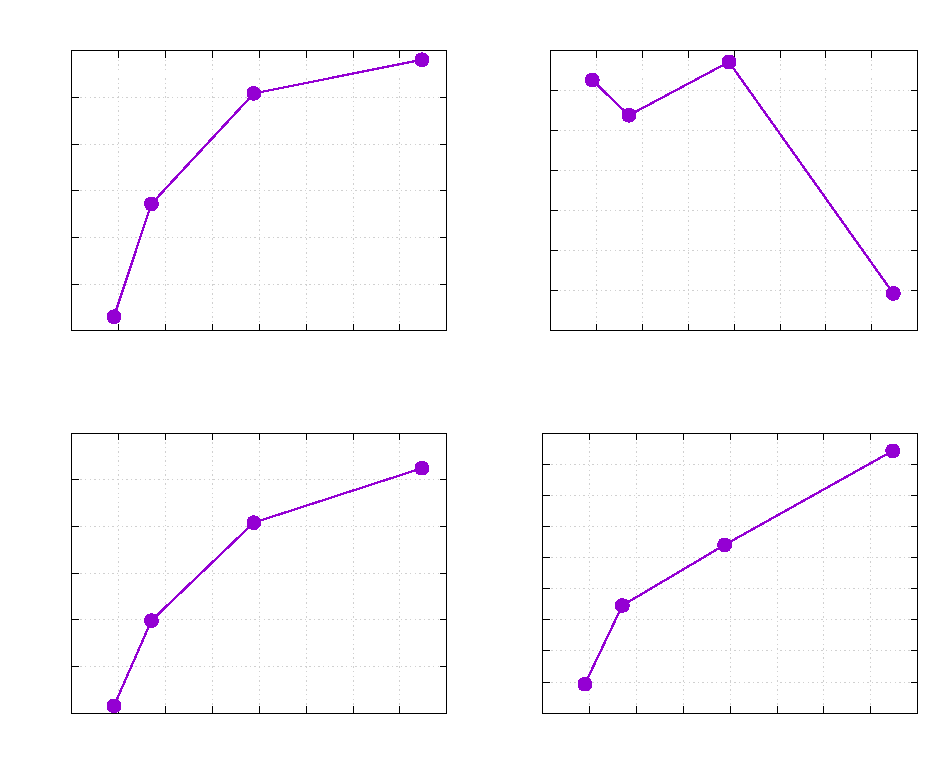
\includegraphics[width={453.00bp},height={368.00bp}]{figures/assignment5_mesh_metrics}}%
    \gplfronttext
  \end{picture}%
\endgroup
